\documentclass[journal]{IEEEtran}
\usepackage{cite}
\usepackage{amsmath,amssymb,amsfonts,mathtools,amsthm}
\usepackage{graphicx}
\usepackage{booktabs,multirow,array,tabularx}
\usepackage{algorithm}
\usepackage{algpseudocode}
\usepackage{siunitx}
\usepackage{balance}
\usepackage[hidelinks]{hyperref}
\usepackage[capitalize,nameinlink]{cleveref}
\usepackage{xurl}
\usepackage{doi}
\usepackage{enumitem}
\usepackage{microtype}
\usepackage{tikz}
\usetikzlibrary{positioning,arrows.meta}
\hypersetup{pdftitle={Shielded Q-learning for Thermally-Safe, Energy-Aware Multi-Model Intrusion Detection Scheduling on Lightweight Edge Devices},pdfauthor={Nuonan Ouyang et al.}}
\newtheorem{proposition}{Proposition}
\newcommand{\Aset}{\mathcal{A}}
\newcommand{\Asafe}{\mathcal{A}_{\mathrm{safe}}}
\newcommand{\E}{\mathbb{E}}
\newcommand{\ind}{\mathbb{I}}
\newcommand{\clipplus}[1]{\left[#1\right]_{+}}
\newcommand{\clipunit}[1]{\left[#1\right]_{0}^{1}}
\newcommand{\tauMax}{40}
\newcommand{\TMax}{82}

\title{Shielded Q-learning for Thermally-Safe, Energy-Aware Multi-Model Intrusion Detection Scheduling on Lightweight Edge Devices}
\author{Nuonan~Ouyang, Adrian~Shatte, Zhigang~Lu, Chao~Chen, and~Wei~Xiang%
\thanks{N. Ouyang (corresponding author) and A. Shatte are with the College of Science and Engineering, James Cook University, Australia (e-mail: nuonan.ouyang@my.jcu.edu.au; adrian.shatte@jcu.edu.au).}%
\thanks{Z. Lu is with the School of Computer, Data and Mathematical Sciences, Western Sydney University, Australia (e-mail: z.lu@westernsydney.edu.au).}%
\thanks{C. Chen is with the School of Accounting, Information Systems \& Supply Chain, RMIT University, Australia (e-mail: chao.chen@rmit.edu.au).}%
\thanks{W. Xiang is with the Australian Centre for AI in Medical Innovation and the Cisco--La Trobe Centre for AI and Internet of Things, La Trobe University, Australia (e-mail: w.xiang@latrobe.edu.au).}%
}
\markboth{IEEE Transactions on Sustainable Computing}{Ouyang \MakeLowercase{et al.}: Shielded Q-learning for Thermally-Safe IDS Scheduling}

\begin{document}
\maketitle

\begin{abstract}
Lightweight edge intrusion detection must balance detection quality with strict latency, thermal, and energy budgets. We formulate multi-model intrusion-detection-system (IDS) scheduling as a constrained Markov decision process and propose Feasible-Set Shielded Q-learning (FSSQL-R): a calibrated runtime guard first restricts model selection to actions predicted to satisfy per-window latency and temperature caps, after which masked Q-learning selects within the admissible set. We evaluate the method through online measurements on Raspberry Pi 3B+ and Raspberry Pi 4B 8GB platforms, with separate device-specific calibration. Held-out guard coverage is 2879/2880 (0.999653) on the Pi 3B+ and 0.998958 joint coverage on the Pi 4B. Under a binding Pi 3B+ regime, the shield excludes LUCID but FSSQL-R does not outperform the simpler Safe-Greedy controller: mean F1 is 0.8523 versus 0.8708 and mean reward is 0.5434 versus 0.5839. In 60 Pi 4B online runs, FSSQL-R improves paired-seed F1 over Safe-Greedy by 0.114--0.121 and cumulative reward by 122--129, but Safe-Greedy is a degenerate reference in this experiment (FPR=1.0000 in every run). A no-training Threshold controller attains the highest mean F1 in all three Pi 4B conditions. Direct POWER-Z KM003C measurements quantify DC input energy, but do not establish a consistent FSSQL-R energy advantage. These results support calibrated feasible-set enforcement while showing that the incremental value of Q-learning is device- and regime-dependent rather than universal.
\end{abstract}

\begin{IEEEkeywords}
Lightweight IoT, intrusion detection, dynamic model scheduling, safe reinforcement learning, shielding, Q-learning, thermal safety, energy measurement, Raspberry Pi.
\end{IEEEkeywords}

\section{Introduction}
Lightweight edge devices increasingly execute intrusion detection close to data sources, but deployability is constrained by latency deadlines, thermal headroom, and energy budgets. The central challenge is not only classification accuracy: a detector that is strong offline can become impractical when sustained execution increases latency, heats the device, or consumes excessive energy \cite{banbury2021mlperftiny,reddi2019mlperfinference,tan2024thermalnpu}. Maintaining a heterogeneous model pool and selecting among detectors online is therefore attractive, particularly when traffic risk and resource state vary over time.

Reinforcement learning (RL) provides a natural mechanism for long-horizon model selection, but unconstrained exploration can violate deployment limits. Constrained MDP approaches typically control expected cost \cite{altman1999cmdp,achiam2017cpo,chow2018lyapunov}, whereas embedded deadlines and temperature limits are operational constraints that may need runtime enforcement. Shielding addresses this by blocking actions that fail an admissibility test before the RL policy acts \cite{alshiekh2018shielding,carr2023partialshielding,koenighofer2025shields}. Recent IDS work has likewise combined a safety-aware RL policy with a runtime shield, although in a 5G self-healing remediation setting rather than resource-constrained detector scheduling \cite{malwi2026safetyaware}.

This paper studies the deployment problem of selecting among heterogeneous on-device IDS models while accounting for detector utility, switching, latency, temperature, and energy. FSSQL-R constructs a calibrated feasible set and applies Q-learning only within that set. We examine whether learning adds practical value beyond the shield, whether the controller is viable in online execution, how a simple threshold controller compares, and how latency, thermal behavior, and measured energy trade off across devices and operating conditions.

The results show that shielding is useful as a device-specific feasibility layer, but Q-learning is not universally superior. On the Pi 3B+, Safe-Greedy outperforms FSSQL-R under a stationary binding regime; on the Pi 4B, FSSQL-R consistently improves F1 and reward over Safe-Greedy, while the no-training Threshold controller has the highest mean F1 in all three evaluated loads. Physical energy differences are small and not consistently significant. We therefore make four contributions:
\begin{enumerate}[leftmargin=*,itemsep=1pt]
\item We formulate the guard as a device-calibrated feasible-set mechanism whose empirical margins constrain action selection without implying an unconditional end-to-end safety guarantee.
\item We compare FSSQL-R with a conventional threshold controller and other baselines using matched-seed analysis, and examine learning stability over 6000 training windows, 1280 states, and 5120 state-action pairs.
\item We evaluate real online closed-loop execution on two Raspberry Pi configurations, including controller and switching overhead, independent device-specific guard calibration, and background-load robustness.
\item We measure DC input-side power and energy directly with a POWER-Z KM003C and evaluate all 82,332 official UNSW-NB15 test rows once using fixed preprocessing and detector thresholds, keeping deployment-workload results separate from independent detector generalization.
\end{enumerate}

\section{Related Work and Positioning}
\subsection{Sustainable scheduling and adaptive edge inference}
Recent work in sustainable computing increasingly treats resource management as an online control problem rather than a static configuration task. In \emph{IEEE Transactions on Sustainable Computing} (TSUSC), Wang \emph{et al.} use deep reinforcement learning (DRL) for runtime GPU frequency capping \cite{wang2024drlcap}; Ko \emph{et al.} schedule energy-harvesting IoT sleep states while preserving reconstruction quality \cite{ko2025rass}; Gao \emph{et al.} jointly optimize latency and energy for in-network task scheduling \cite{gao2025inc}; and Li \emph{et al.} learn DVFS policies for multitask edge workloads under deadlines \cite{li2025dvfsedge}. Recent TSUSC work also highlights adaptation in IoT anomaly detection under concept drift \cite{xu2024conceptdrift}. These studies motivate dynamic resource-aware control, but their actions are frequency, sleep, task-placement, or adaptation decisions rather than selection among heterogeneous on-device IDS models.

Closely related edge-inference work in \emph{IEEE Transactions on Mobile Computing} (TMC) reinforces the need to account for workload variation and the cost of the controller itself. Tan \emph{et al.} formulate workload-adaptive edge inference request scheduling as an MDP and use RL to select among model-serving choices \cite{tan2024workloadadaptive}; Zhang \emph{et al.} co-optimize DVFS and edge-cloud offloading for latency/energy efficiency \cite{zhang2024dvfo}; and thermal-aware scheduling has been studied explicitly for mobile DNN execution \cite{tan2024thermalnpu}. Our problem differs in two respects: model selection is constrained by a separately calibrated per-window feasible set, and the revised evaluation measures complete online controller latency and physical input energy on the target device rather than relying only on a modeled cost.

\subsection{Lightweight and online intrusion detection}
Lightweight IDS research spans classical one-class methods, extreme learning machines, compact deep models, and TinyML-style deployment \cite{tax2004svdd,huang2006elm,doriguzzi2020lucid,fusco2024tinyids,warden2019tinyml,lin2020mcunet}. More recent high-end security literature has emphasized adaptation as well as compact execution. Nakip and Gelenbe propose an online self-supervised IDS that adapts without conventional offline relabeling \cite{nakip2024selfsupervised}, while Yang \emph{et al.} address lightweight dynamic open-set intrusion detection for IIoT \cite{yang2025openset}. These works focus on improving or updating the detector. The practical problem here is complementary: the detectors are frozen before formal evaluation, and the runtime controller decides which detector to execute under latency, thermal, and resource constraints.

\subsection{Safe RL and shielding}
Safe RL covers expectation-constrained optimization, Lyapunov methods, and action shielding \cite{garcia2015safesurvey,achiam2017cpo,chow2018lyapunov,alshiekh2018shielding}. FSSQL-R is not novel because shielding itself is new; rather, it instantiates a calibrated, device-specific feasible-action layer for multi-model IDS scheduling and separates this layer from utility optimization. Malwi \emph{et al.} \cite{malwi2026safetyaware} use a runtime safety shield for self-healing remediation actions in 5G-IoT. Our action semantics and constraints are different: the actions are heterogeneous IDS models, and admissibility is derived from device-specific latency and thermal measurements under explicit operating caps.

\subsection{Positioning against simpler controllers}
A key lesson from the revision is that learning must be compared with controllers that do not require training. The baseline set therefore includes Static-Light, Round-Robin, Safe-Greedy, Unshielded-Q, and a conventional threshold controller. Safe-Greedy uses the same calibrated feasible set as FSSQL-R but makes a one-step security-utility choice. Unshielded-Q uses the same state, reward, and Q-learning implementation without feasible-set masking. The threshold controller uses only measured state and fixed development-time thresholds. Earlier energy-aware and multi-objective precursor formulations are not archival publications and are not used to establish novelty. The numeric Q-learning configuration used here is reported explicitly, fixed before formal evaluation, and evaluated against these simpler alternatives.

\begin{table*}[t]
\caption{Recent work most closely related to sustainable scheduling, edge inference, and adaptive IDS.}
\label{tab:recentwork}
\centering\scriptsize
\begin{tabularx}{\textwidth}{@{}p{2.45cm}p{2.15cm}p{3.0cm}p{3.35cm}>{\raggedright\arraybackslash}X@{}}
\toprule
Work & Venue & Runtime decision & Main evidence/constraint & Relation to this work \\
\midrule
Wang \emph{et al.} \cite{wang2024drlcap} & TSUSC 2024 & GPU frequency cap & DRL-based runtime power control & Sustainable runtime control; no IDS feasible-set guard \\
Xu \emph{et al.} \cite{xu2024conceptdrift} & TSUSC 2024 & Drift adaptation & IoT anomaly adaptation across datasets & Adaptive security model rather than detector scheduling \\
Ko \emph{et al.} \cite{ko2025rass} & TSUSC 2025 & IoT sleep scheduling & Energy harvesting and outage-aware DRL & Energy-aware IoT control; different action and constraint semantics \\
Gao \emph{et al.} \cite{gao2025inc} & TSUSC 2025 & In-network task scheduling & Joint latency/energy optimization & Related multi-objective scheduling, primarily network/compute placement \\
Li \emph{et al.} \cite{li2025dvfsedge} & TSUSC 2025 & DVFS selection & Deadline-aware edge execution & Device adaptation through frequency, not IDS model selection \\
Tan \emph{et al.} \cite{tan2024workloadadaptive} & TMC 2024 & Edge inference requests/models & Workload-adaptive RL scheduling & Closest adaptive inference framing; no calibrated IDS shield \\
Zhang \emph{et al.} \cite{zhang2024dvfo} & TMC 2024 & DVFS + offloading & Physical heterogeneous edge evaluation & Latency/energy control through DVFS/offloading \\
Nakip and Gelenbe \cite{nakip2024selfsupervised}; Yang \emph{et al.} \cite{yang2025openset} & TIFS 2024--25 & Online/open-set IDS adaptation & Dynamic IDS learning and lightweight execution & Improves detector adaptation; our focus is constrained runtime selection among frozen detectors \\
\textbf{This work} & TSUSC & IDS model selection & Device-calibrated latency/thermal guard, complete online timing, direct DC input energy & Higher-level complement to DVFS/power control; no consistent energy-saving claim \\
\bottomrule
\end{tabularx}
\end{table*}

\section{Problem Formulation}
We consider fixed decision windows of length $\Delta=100$ ms. An action $a_t\in\Aset=\{1,\ldots,K\}$ selects one of $K=4$ frozen IDS models. The state is
\begin{equation}
s_t=(z_t,T_t,b_t,q_t,a_{t-1}),
\label{eq:state}
\end{equation}
where $z_t$ is a lightweight risk/workload descriptor, $T_t$ is CPU temperature, $b_t$ is a normalized energy-state proxy used by the controller reward, $q_t$ is backlog state, and $a_{t-1}$ captures switching history.

The per-window utility is
\begin{equation}
\begin{split}
r_t = r_{\rm sec}(z_t,a_t)-\lambda_E e(a_t)
-\lambda_Q\psi(q_t)-\lambda_S c_{\rm sw}(a_{t-1},a_t),
\end{split}
\label{eq:reward}
\end{equation}
where $r_{\rm sec}$ combines the risk estimate with fixed validation TPR/FPR, and the remaining terms penalize compute/energy proxy, backlog, and switching. The deployment constraints are
\begin{equation}
\tau(s_t,a_t)\le \tau_{\max}=40\;\text{ms},\qquad
T_{t+1}(s_t,a_t)\le T_{\max}=82^\circ\text{C}.
\label{eq:caps}
\end{equation}

Let $\widehat{\tau}(s,a)$ and $\widehat{T}_{t+1}(s,a)$ be device-calibrated one-step predictors. With one-sided residual margins $\epsilon_{\tau,a}$ and $\epsilon_T$, the feasible set is
\begin{equation}
\begin{split}
\Asafe(s)=\{a\in\Aset:\;&\widehat{\tau}(s,a)+\epsilon_{\tau,a}\le\tau_{\max},\\
&\widehat{T}_{t+1}(s,a)+\epsilon_T\le T_{\max}\}.
\end{split}
\label{eq:safeset}
\end{equation}
If $\Asafe$ is nonempty, FSSQL-R chooses the maximizing Q action inside this set. Empty-set handling uses the fixed least-violating fallback, although no fallback occurred in the accepted formal online campaigns.

\section{Feasible-Set Shielded Q-learning}
\subsection{Calibrated guard}
The guard is calibrated separately for each hardware configuration. Latency uses per-action/workload/background empirical predictors; thermal prediction uses a fitted one-step model. Predictor fitting, residual-margin estimation, and held-out coverage evaluation are separated. We use a Q0.99 one-sided residual margin with a fixed conservative buffer selected before held-out coverage is evaluated.

\subsection{Masked Q-learning}
For a nonterminal transition $(s_t,a_t,r_t,s_{t+1})$, the update is
\begin{equation}
\begin{split}
Q(s_t,a_t)\leftarrow Q(s_t,a_t)+\alpha_t\big[&r_t+\gamma \max_{a'\in\Asafe(s_{t+1})}Q(s_{t+1},a')\\
&-Q(s_t,a_t)\big].
\end{split}
\label{eq:q}
\end{equation}
The implementation has 1280 discretized states and 5120 state-action pairs. We use $\gamma=0.95$, $\alpha=\min\{0.5,(1+N(s,a))^{-0.6}\}$, and linearly decay $\epsilon$ from 1.0 to 0.05 by window 4500, retaining 0.05 thereafter. A FIFO replay buffer of 512 transitions performs one online update plus four uniformly sampled replay updates per training window. Formal evaluation uses $\epsilon=0$ and disables Q/replay updates.

\subsection{Conditional safety statement}
The safety result is conditional rather than absolute.
\begin{proposition}[Conditional one-step admissibility]
If the true latency and next-temperature errors are bounded by the calibrated guard margins for a state-action pair, every action admitted by \eqref{eq:safeset} satisfies the modeled one-step caps in \eqref{eq:caps}.
\end{proposition}
\begin{proof}
For an admitted action, $\widehat{\tau}+\epsilon_{\tau,a}\le\tau_{\max}$ and $\widehat{T}_{t+1}+\epsilon_T\le T_{\max}$. If the corresponding positive prediction errors do not exceed the margins, the true quantities are bounded by the same cap. \qed
\end{proof}
The empirical residual distribution can violate this assumption. Moreover, complete end-to-end latency includes controller/runtime effects beyond the modeled detector/service component. We therefore report held-out coverage and realized online violations explicitly rather than describing the calibration as an unconditional guarantee.

\section{Experimental Method}
\subsection{Data and model pool}
We use UNSW-NB15 \cite{moustafa2015unsw}. The official training file is split into group-safe development partitions for model training, validation, and scheduler development. All detector-quality terms used by the scheduler reward are fixed from the validation partition; official-test statistics do not enter model training, guard calibration, reward construction, Q-learning, or policy selection. The official 82,332-row test set is sealed throughout calibration, scheduler training, hardware experiments, and statistical analysis, then opened once for the final detector-generalization evaluation. The fixed action pool is FISVDD, LUCID, TinyDL, and OI-SVDD+AS-ELM.

\subsection{Hardware and calibration}
We evaluate a Raspberry Pi 3 Model B+ and a Raspberry Pi 4 Model B with 8 GB RAM. The Pi 3B+ is operated with a heatsink and continuously active fan inside an open-top case, with a stabilized wall-powered supply path; the Pi 4B uses active cooling. Accepted formal runs use the \texttt{performance} governor and reject current throttling/undervoltage events or frequency violations. The two devices are calibrated independently; Pi 3B+ predictor/margin artifacts are never reused on the Pi 4B.

\begin{table}[t]
\caption{Consolidated experimental parameters.}
\label{tab:params}
\centering\footnotesize
\begin{tabularx}{\columnwidth}{@{}l>{\raggedright\arraybackslash}X@{}}
\toprule
Parameter & Value \\
\midrule
Decision window & 100 ms \\
Latency cap $\tau_{\max}$ & 40 ms \\
Thermal cap $T_{\max}$ & $82^\circ$C \\
Actions & 4 IDS models \\
Q states / state-actions & 1280 / 5120 \\
Discount $\gamma$ & 0.95 \\
Replay capacity & 512 \\
Pi 3B+ binding matrix & 6 policies $\times$ 10 seeds $\times$ 600 windows \\
Pi 4B online matrix & 4 policies $\times$ 3 loads $\times$ 5 seeds $\times$ 600 windows \\
Pi 4B loads & $n=16$, B0/B1/B2 background CPU \\
Energy meter & POWER-Z KM003C, direct HID \\
Energy boundary & DC input side of Pi 4B power path \\
\bottomrule
\end{tabularx}
\end{table}

Calibration uses 72 action/workload/background cells (4 actions $\times$ 6 batch sizes $\times$ 3 background conditions) with separate fit, margin, and held-out coverage splits, each containing 2880 windows. Table~\ref{tab:coverage} reports the accepted held-out coverage.

\begin{table}[t]
\caption{Held-out empirical guard coverage (no post-coverage tuning).}
\label{tab:coverage}
\centering\footnotesize
\begin{tabular}{lccc}
\toprule
Device & Latency & Thermal & Joint \\
\midrule
Pi 3B+ & 0.999653 & 1.000000 & 0.999653 \\
Pi 4B 8GB & 1.000000 & 0.998958 & 0.998958 \\
\bottomrule
\end{tabular}
\end{table}

\subsection{Evidence separation and runtime accounting}
The evaluation separates four evidence roles that can otherwise be conflated in adaptive systems. First, detector fitting and scheduler development use only the official UNSW-NB15 training file. Ground-truth labels associated with the frozen scheduler-development workload are held as a scoring sidecar: they are unavailable to preprocessing, risk estimation, state construction, guard evaluation, reward construction, Q-learning, and action selection, and are joined only after the selected detector has produced a prediction. Second, guard calibration uses disjoint fit, margin, and coverage windows on each device, and coverage observations never modify the accepted predictor or margin. Third, formal online policy comparisons use frozen device-specific guard/Q artifacts and fixed run orders. Finally, the official test file is opened only after all development-side choices and hardware analyses are frozen.

We distinguish action/service latency from complete online latency. The guard predicts the service component associated with executing a candidate detector under the calibrated workload/background state. The formal worker separately measures preprocessing, telemetry, state construction, guard/admissible-set evaluation, policy selection, detector inference, switching, and complete end-to-end (E2E) elapsed time using the Pi monotonic clock. This separation is necessary because a detector can satisfy the calibrated service bound while operating-system or controller jitter creates an E2E tail event. The controller is therefore treated as part of the deployment cost rather than assumed negligible.

For Pi 4B energy measurements, KM003C acquisition runs on the Mac orchestrator and does not enter the Pi controller critical path. Meter samples and run-boundary acknowledgements share the Mac monotonic clock domain; Pi monotonic timestamps are used only for internal latency accounting. Raw meter traces include pre/post roll and are integrated over the acknowledged run boundaries. Technical acquisition failures are retained as failed attempts rather than silently overwritten; only the predefined technically valid replacement attempt enters the accepted scientific cell.

\subsection{Baselines and online execution}
Safe-Greedy uses the same $\Asafe$ as FSSQL-R but maximizes current security utility without temporal learning. Unshielded-Q removes feasible-set masking. Static-Light fixes the light action. Round-Robin cycles through the pool. The added no-training Threshold controller uses development-calibrated temperature/backlog/risk thresholds: high temperature or backlog selects the light action; sufficiently cool/low-backlog high-risk state selects the highest-validation-utility action; otherwise it retains the previous action.

On the Pi 3B+, a stationary binding-resource matrix compares six policies over 10 matched seeds. The accepted guard has $|\Asafe|=3$ in every window and excludes LUCID. On the Pi 4B, we run 60 complete online experiments: FSSQL-R, Safe-Greedy, Threshold, and Static-Light under B0, B1, and B2 background load, with five matched seeds and 600 windows per run. Every window records preprocessing, telemetry, state construction, guard/admissible-set construction, policy selection, Q lookup, detector inference, switching, total controller time, complete end-to-end latency, temperature, frequency, fault flags, action, and post-action confusion-matrix contributions.

\subsection{Physical energy measurement}
A POWER-Z KM003C measures the Pi 4B DC input path at approximately 10 samples/s. Each formal run includes at least 5 s pre-roll and 5 s post-roll. Energy is computed by trapezoidal integration of measured power using actual Mac monotonic timestamps over the run ACK boundaries. Two initial runs with invalid meter binding were preserved as technical failures and repeated under the predefined technical invalidation rule; the accepted set contains 60 complete scientific cells and 36,000 windows. Primary energy results are absolute input energy without idle subtraction.

\subsection{Statistics}
The statistical unit is the matched run/seed, never a pooled window. Pi 3B+ paired comparisons use 10 matched seeds; Pi 4B uses five matched seeds per condition. We report raw paired values, mean/SD, bootstrap 95\% CIs for mean differences, paired tests, and effect sizes. Because $n=5$ limits exact nonparametric power, we report both paired $t$ and exact Wilcoxon results for the Pi 4B comparison rather than treating one test as definitive.

\section{Results}
\subsection{RQ1: Does calibrated shielding create a meaningful feasible set?}
The Pi 3B+ held-out joint coverage is 2879/2880 (0.999653); the single uncovered point is retained. Under the binding-resource experiment, the guard excludes LUCID and maintains exactly three admissible actions in all 36,000 windows. Thus, on this constrained device the shield actively changes the action set. In contrast, all Pi 4B online windows retain all four actions ($|\Asafe|=4$). This cross-device result shows why calibration is hardware-specific: the same 40-ms operating cap is binding on the Pi 3B+ workload but nonbinding on the stronger Pi 4B for the evaluated online conditions.

One Pi 3B+ Threshold window exceeds the 40-ms complete E2E cap (52.522 ms) despite the selected TinyDL action having a guarded predicted latency of 5.147 ms with 24.297 ms headroom. Detector inference is only 0.446 ms; the event is dominated by a 50.414-ms controller/runtime outlier. This retained event motivates the claim boundary: the guard calibrates modeled action/service latency and thermal feasibility, while complete pipeline timing must be measured empirically.

\subsection{RQ2: Does Q-learning add value over Safe-Greedy?}
Table~\ref{tab:pi3} reports the Pi 3B+ binding regime. In this regime, FSSQL-R does not improve on Safe-Greedy. Its mean F1 and reward are lower, mean E2E latency is higher, and switching is substantially greater; both methods have zero realized violations. Exact paired sign-flip tests give $p=0.00195$ for F1, reward, and switching cost, and $p=0.00586$ for mean E2E latency. The mean controller-overhead difference is not significant ($p=0.23242$).

\begin{table}[t]
\caption{Pi 3B+ binding-resource results, mean over 10 matched seeds.}
\label{tab:pi3}
\centering\footnotesize
\begin{tabular}{lrrrrr}
\toprule
Policy & F1 & Reward & E2E ms & Switch cost & Viol. \\
\midrule
FSSQL-R & 0.8523 & 0.5434 & 8.3149 & 5.348 & 0 \\
Safe-Greedy & \textbf{0.8708} & \textbf{0.5839} & \textbf{7.9775} & \textbf{0} & 0 \\
Threshold & 0.8704 & 0.5834 & 7.9704 & 0.012 & 1 \\
Unshielded-Q & 0.8523 & 0.5489 & 10.1141 & 4.438 & 0 \\
Round-Robin & 0.8148 & 0.4801 & 10.6571 & 11.980 & 0 \\
Static-Light & 0.7203 & 0.3389 & 8.2550 & 0 & 0 \\
\bottomrule
\end{tabular}
\end{table}

A predefined stateful-transition extension was stopped before policy evaluation because measured action service rates could not simultaneously establish the required backlog accumulation under B2/B1 and recovery under B0 without inventing a new arrival-rate rule. We therefore do not use it as evidence for or against Q-learning.

On Pi 4B, the result differs, but the comparison requires an important qualification. Table~\ref{tab:pi4} shows higher F1 and cumulative reward for FSSQL-R than Safe-Greedy under all three background loads. However, Safe-Greedy collapses to FISVDD in all 15 formal runs and consequently has $\mathrm{FPR}=1.0000$ and $\mathrm{TN}=0$ in every run. We retain it because it is the direct same-guard, one-step reference, but it represents an extreme operating point rather than a competitive detector selector. The paired F1 mean differences are +0.1209 (B0), +0.1172 (B1), and +0.1141 (B2), with bootstrap 95\% CIs that remain positive; paired $t$-test $p$ values are 0.011--0.015 and exact Wilcoxon $p=0.0625$ in each condition. We therefore describe this as a consistent paired advantage over Safe-Greedy, not as overall superiority.

\begin{table*}[t]
\caption{Pi 4B 8GB online results across five matched seeds per condition. F1, reward, latency, controller time and energy are mean $\pm$ SD; FPR is median [min,max] because its seed distribution is strongly non-Gaussian.}
\label{tab:pi4}
\centering\scriptsize
\setlength{\tabcolsep}{2.2pt}
\begin{tabular}{llccccccc}
\toprule
Load & Policy & F1 & FPR med. [range] & Cum. reward & P99 E2E (ms) & Controller (ms) & Energy (J) & Viol. \\
\midrule
B0 & FSSQL-R & $0.9235\pm0.0534$ & $0.1917$ [0.0674,0.9144] & $333.8\pm52.2$ & $5.386\pm0.151$ & $3.909\pm0.164$ & $173.93\pm12.46$ & 0 \\
B0 & Safe-Greedy & $0.8025\pm0.0117$ & $1.0000$ [1.0000,1.0000] & $204.4\pm19.5$ & $5.063\pm0.279$ & $3.872\pm0.023$ & $174.40\pm9.42$ & 0 \\
B0 & Static-Light & $0.9332\pm0.0120$ & $0.2190$ [0.1865,0.2767] & $346.2\pm17.9$ & $5.727\pm0.936$ & $4.114\pm0.170$ & $175.47\pm19.98$ & 0 \\
B0 & Threshold & $\mathbf{0.9491\pm0.0117}$ & $\mathbf{0.0714}$ [0.0622,0.0874] & $\mathbf{362.0\pm16.5}$ & $5.436\pm1.118$ & $3.834\pm0.189$ & $183.66\pm6.24$ & 0 \\
\midrule
B1 & FSSQL-R & $0.9271\pm0.0580$ & $0.1869$ [0.0444,0.9780] & $341.6\pm58.3$ & $5.021\pm0.328$ & $3.897\pm0.156$ & $164.50\pm0.58$ & 0 \\
B1 & Safe-Greedy & $0.8099\pm0.0117$ & $1.0000$ [1.0000,1.0000] & $216.8\pm19.9$ & $5.150\pm0.542$ & $3.879\pm0.066$ & $167.93\pm3.85$ & 0 \\
B1 & Static-Light & $0.9387\pm0.0065$ & $0.2278$ [0.1832,0.2602] & $356.2\pm9.5$ & $5.481\pm0.223$ & $4.075\pm0.019$ & $168.80\pm5.08$ & 0 \\
B1 & Threshold & $\mathbf{0.9533\pm0.0106}$ & $\mathbf{0.0444}$ [0.0354,0.1173] & $\mathbf{371.0\pm15.1}$ & $7.927\pm5.707$ & $4.258\pm1.067$ & $181.38\pm10.36$ & 1 \\
\midrule
B2 & FSSQL-R & $0.9222\pm0.0711$ & $0.1882$ [0.0378,0.9476] & $336.0\pm83.5$ & $5.352\pm0.576$ & $3.951\pm0.119$ & $171.32\pm8.16$ & 0 \\
B2 & Safe-Greedy & $0.8081\pm0.0199$ & $1.0000$ [1.0000,1.0000] & $214.0\pm33.8$ & $5.318\pm0.573$ & $3.905\pm0.093$ & $172.53\pm8.11$ & 0 \\
B2 & Static-Light & $0.9374\pm0.0071$ & $0.2270$ [0.1832,0.2381] & $354.2\pm21.1$ & $8.919\pm7.298$ & $4.643\pm1.193$ & $175.17\pm21.45$ & 1 \\
B2 & Threshold & $\mathbf{0.9627\pm0.0040}$ & $\mathbf{0.0471}$ [0.0378,0.0647] & $\mathbf{377.0\pm13.6}$ & $\mathbf{4.913\pm0.283}$ & $\mathbf{3.747\pm0.026}$ & $168.24\pm4.56$ & 0 \\
\bottomrule
\end{tabular}
\end{table*}

These results also answer the request for a simple controller. Threshold is the strongest detector-selection baseline by mean F1 in all three Pi 4B conditions, and it also has much lower mean FPR (0.0726/0.0581/0.0490 for B0/B1/B2) than FSSQL-R (0.2936/0.3060/0.3109). The FSSQL-R mean, however, masks a reproducible seed-specific failure mode: seed 5102 selects FISVDD in 582/600, 592/600, and 588/600 windows under B0/B1/B2, yielding FPR 0.9144/0.9780/0.9476 and F1 0.8285/0.8245/0.7967. The other four seeds have mean FPR 0.1384/0.1380/0.1517, still above Threshold. Table~\ref{tab:pi4} therefore reports FPR as median [range], and the supplement gives all five seed-level values. For the paired FSSQL-R-minus-Threshold FPR differences, the bootstrap 95\% CIs are [+0.0249,+0.5384], [+0.0323,+0.5928], and [+0.0581,+0.5896], respectively; the corresponding F1-difference intervals cross zero. Given only five pairs, the paired $t$ and Wilcoxon tests for FPR do not cross 0.05, so we interpret the positive bootstrap intervals as directional evidence rather than a universal significance claim. Safe-Greedy is retained because it isolates the one-step same-guard decision rule, but its FPR=1.0000/TN=0 behavior makes it a degenerate detector-selection reference in this Pi 4B experiment. FSSQL-R therefore should not be interpreted as an overall winner.

\subsection{Learning stability and complexity}
At 600 training windows, FSSQL-R has mean rolling reward 0.4837, utility 0.5759, and visits 29.7 states/96.3 state-action pairs. At 6000 windows, these become 0.5260, 0.6108, and 34.9/118.9. The greedy-policy change rate falls from 0.006875 to 0.000156. Unshielded-Q shows a similar reduction. Because state support remains sparse and the absolute TD error remains nonzero, this evidence supports late-budget behavioral stability over visited states, not mathematical convergence over the complete 1280-state space.

\subsection{RQ3: What is the measured deployment cost?}
Controller work is material relative to detector inference. Across all Pi 4B conditions, mean controller time is 3.919 ms for FSSQL-R and 3.885 ms for Safe-Greedy, whereas mean selected-detector inference is about 0.415 and 0.426 ms, respectively. Thus, telemetry/state/guard/policy logic must be included when assessing deployment cost. FSSQL-R also switches more often (mean 26.8 switches/run across the three conditions) than Safe-Greedy (zero under the fixed utility rule).

Physical power results are shown in Fig.~\ref{fig:energy}. The FSSQL-R minus Safe-Greedy paired mean energy differences are $-0.471$ J (B0), $-3.427$ J (B1), and $-1.210$ J (B2). These differences do not provide consistent statistical evidence for a physical energy advantage: B0/B2 CIs span zero, and the B1 exact Wilcoxon result is $p=0.0625$. We therefore report energy as a measured operating trade-off rather than a demonstrated energy saving.

\begin{figure}[t]
\centering
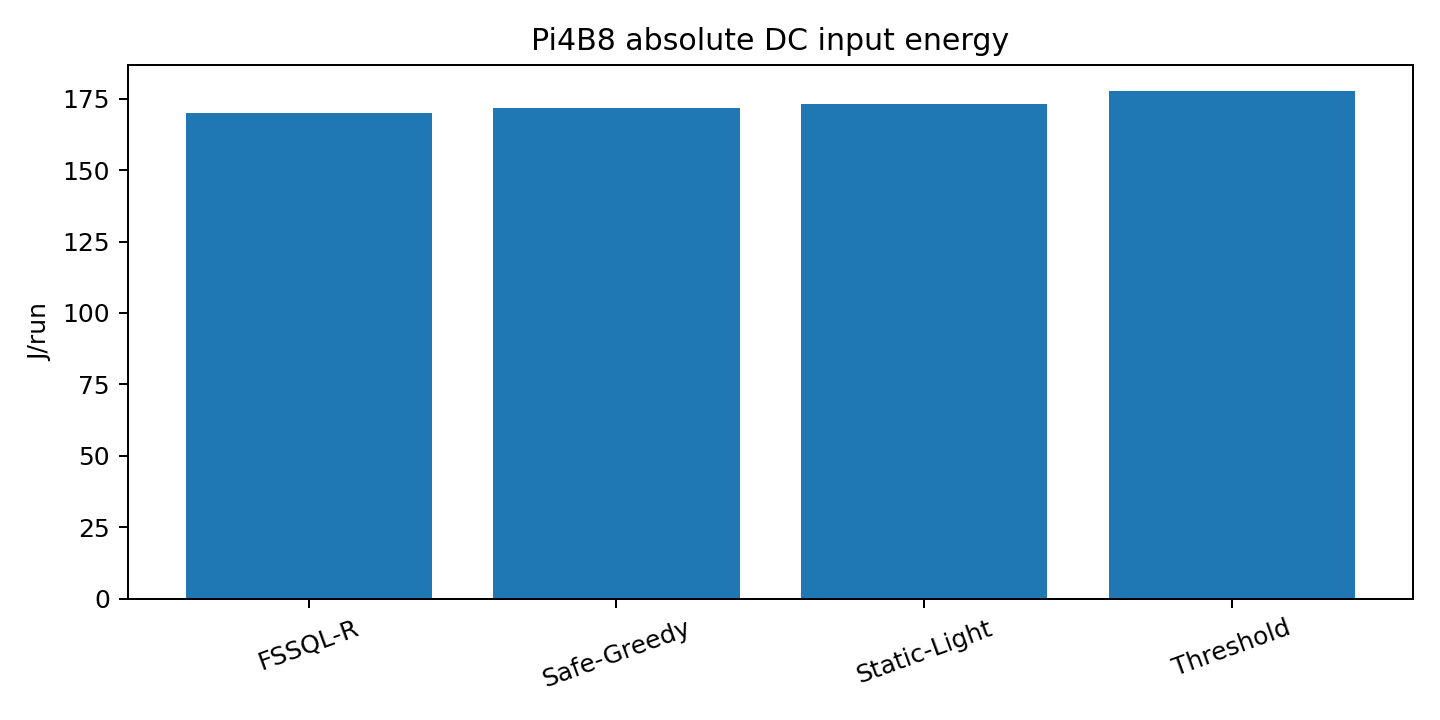
\includegraphics[width=\columnwidth]{figures/PI4B8_POWER_ENERGY_COMPARISON.png}
\caption{Absolute Pi 4B DC input energy measured by POWER-Z KM003C. Bars aggregate the accepted formal online runs; absolute input energy is reported without idle subtraction.}
\label{fig:energy}
\end{figure}

\begin{figure*}[t]
\centering
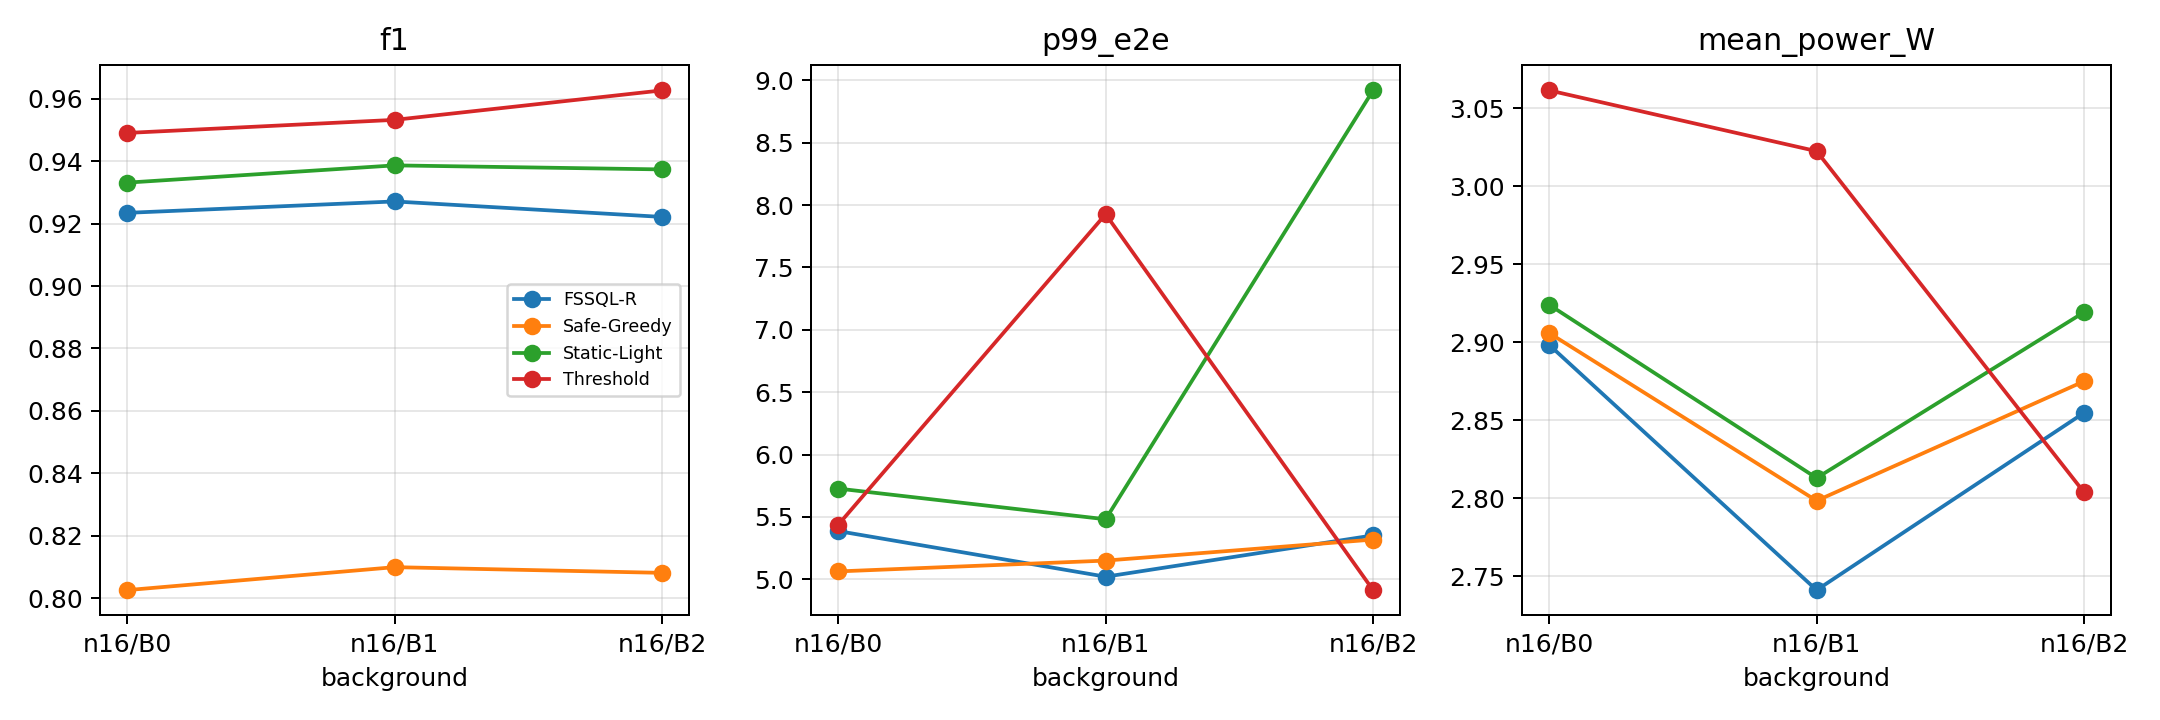
\includegraphics[width=0.95\textwidth]{figures/PI4B8_B0_B1_B2_ROBUSTNESS.png}
\caption{Pi 4B robustness across B0/B1/B2 background CPU load. F1 is comparatively stable; controller/E2E tails show occasional operating-system/runtime variability, while average DC input power changes modestly.}
\label{fig:robust}
\end{figure*}

\subsection{RQ4: Independent detector generalization}
After model, preprocessing, threshold, and scheduling choices were fixed, the official UNSW-NB15 test was evaluated once on all 82,332 rows. Table~\ref{tab:test} reports independent detector generalization. TinyDL provides the best F1 (0.8686) and the best AUROC/PR-AUC. FISVDD is retained as an adverse result: at its frozen threshold it predicts all test rows positive, yielding recall 1.0 but FPR 1.0; its AUROC is only 0.5351, indicating near-random ranking ability rather than threshold misalignment alone. By contrast, TinyDL and OI-SVDD+AS-ELM achieve AUROC 0.9704 and 0.9513, respectively. These test results are not mixed with the Pi 4B scheduler-development online F1 values.

\begin{table}[t]
\caption{Official UNSW-NB15 test with fixed thresholds (82,332 rows).}
\label{tab:test}
\centering\footnotesize
\begin{tabular}{lrrrr}
\toprule
Detector & F1 & Precision & Recall & FPR \\
\midrule
FISVDD & 0.7102 & 0.5506 & 1.0000 & 1.0000 \\
LUCID & 0.8240 & 0.7020 & 0.9973 & 0.5186 \\
TinyDL & \textbf{0.8686} & \textbf{0.7802} & 0.9797 & \textbf{0.3382} \\
OI-SVDD+AS-ELM & 0.8521 & 0.7437 & \textbf{0.9975} & 0.4211 \\
\bottomrule
\end{tabular}
\end{table}

\section{Discussion}
\subsection{What the shield establishes}
The strongest repeatable conclusion is the calibrated feasibility mechanism. On the Pi 3B+ binding workload, the guard changes the action set by excluding LUCID; on the Pi 4B, the same operating cap is nonbinding under the evaluated online loads. The shield is therefore not universally ``necessary for safety.'' Rather, it provides a device-calibrated mechanism for preventing an adaptive policy from selecting actions that are predicted to exceed the calibrated operating envelope when that envelope becomes binding.

\subsection{When is Q-learning worth its complexity?}
The two devices do not support a universal answer. In the stationary Pi 3B+ binding regime, learning adds switching cost and reduces F1/reward relative to Safe-Greedy. On Pi 4B, FSSQL-R consistently improves F1 and reward over Safe-Greedy, but Threshold has the highest mean F1 and lowest mean FPR in all three loads, while Static-Light also remains strong. The Pi 4B seed-level results additionally expose a reproducible failure mode: one of five FSSQL-R training seeds (5102) produces a stable FISVDD-dominated evaluation policy in all three loads and yields near-all-positive FPR, whereas the other four seeds remain far lower. With only five seeds this 1/5 observation is not a population failure-rate estimate, but it shows why learning-based schedulers should report per-seed policy behavior and action support rather than only mean performance. A predefined queue-state extension could not establish the required accumulation/recovery dynamics and was stopped before policy runs. Consequently, we do not claim that long-horizon RL is always required; the evidence indicates that its value is operating-regime dependent and seed-sensitive.

\subsection{Sustainability interpretation}
We directly measure DC input energy rather than relying on a normalized proxy. This closes an important deployment-evidence gap but changes the claim: FSSQL-R does not demonstrate a consistent physical energy saving. Sustainability is therefore interpreted as measured operation under latency/thermal constraints with explicit energy accounting, not as a guaranteed reduction in joules.

\subsection{Relation to recent sustainable edge control}
The recent TSUSC literature shows several successful uses of learning for energy- or resource-aware scheduling, but it also illustrates that the control variable and measurement boundary matter. DRLCap controls GPU frequency at runtime \cite{wang2024drlcap}; RASS schedules energy-harvesting IoT sleep states \cite{ko2025rass}; latency/energy-aware in-network scheduling jointly allocates communication and computation resources \cite{gao2025inc}; and DRL-based DVFS adapts processor frequency for multitask edge systems \cite{li2025dvfsedge}. These mechanisms directly manipulate a resource with a strong first-order effect on power or service capacity. FSSQL-R instead chooses among already trained IDS models while leaving the hardware governor fixed during formal evaluation. It is therefore plausible for FSSQL-R to change F1 and reward without producing a large or statistically stable change in whole-device input energy. The direct KM003C result is consequently important not because it confirms an energy-saving hypothesis, but because it prevents a controller-internal energy proxy from being interpreted as a physical joule reduction.

The edge-inference literature makes a related point from a performance perspective. Workload-adaptive scheduling \cite{tan2024workloadadaptive}, DVFS/offloading co-optimization \cite{zhang2024dvfo}, and thermal-aware mobile inference \cite{tan2024thermalnpu} all exploit platform state to change a serving configuration. Our cross-device result adds a complementary observation: the same nominal 40-ms cap can be binding on a Pi 3B+ and nonbinding on a Pi 4B, so the practical value of a shield depends on the calibrated platform and workload rather than only on the policy design. This is also why a device-specific guard is preferable to transferring margins across hardware.

\subsection{Implications for deployable IDS}
Recent TIFS work demonstrates that online adaptation and open-set handling can improve the robustness of IoT/IIoT intrusion detection \cite{nakip2024selfsupervised,yang2025openset}. Our results identify a different deployment bottleneck: when several competent detectors are already available, the scheduling layer and its telemetry/decision path can become a nontrivial part of total latency. On Pi 4B the mean controller cost is an order of magnitude larger than selected-detector inference for some actions, and the retained Pi 3B+ tail event is dominated by controller/runtime delay rather than classifier execution. A lightweight IDS scheduler should therefore be evaluated as a complete online system rather than by detector latency alone.

The strong Threshold and Static-Light results also have a practical implication. Learning should be retained only where the operating regime provides enough variation for the additional state/action complexity to pay for itself. The Pi 3B+ stationary binding experiment favors Safe-Greedy, while Pi 4B favors FSSQL-R over Safe-Greedy but not over every simple baseline. This suggests a deployment hierarchy: first calibrate a feasible set, then compare a low-overhead deterministic controller with a learned controller under matched online conditions, and adopt Q-learning only if its incremental detection/utility gain justifies switching and controller cost. Such a hierarchy is consistent with the broader sustainable-computing objective of avoiding unnecessary computation rather than treating learning complexity as intrinsically beneficial.

\section{Limitations and Threats to Validity}
First, both hardware platforms are Raspberry Pi-class devices; MCU applicability remains prospective. Second, guard coverage is empirical and device/configuration dependent. The 0.999653 and 0.998958 joint coverage values are strong held-out evidence but not mathematical guarantees against all runtime tails. Third, complete E2E latency includes controller and operating-system effects that are not fully represented by the action-level guard; the retained Pi 3B+ controller outlier illustrates this boundary. Fourth, the Pi 4B online F1 values are measured on a fixed labeled scheduler-development workload and are intended for matched deployment comparison, not independent generalization. The official test results in Table~\ref{tab:test} provide the independent detector-generalization evidence. Fifth, only five matched Pi 4B seeds are available per condition, limiting exact nonparametric power. The repeated seed-5102 FPR collapse is therefore reported as an observed seed-specific failure mode, not as an estimate of its population probability. Finally, the original experimental artifacts were unavailable. The detector, preprocessing, calibration, and scheduling artifacts used in this revision were therefore reconstructed from the submitted method definitions and frozen before evaluation; they are not claimed to be byte-identical historical artifacts, and the revised empirical tables replace rather than numerically reproduce the earlier replay tables. The Q-learning configuration reported here was likewise fixed before the new experiments and is documented explicitly. The conclusions apply to this configuration.

\section{Conclusion}
This work studies multi-model IDS scheduling under explicit latency and thermal operating limits. FSSQL-R separates calibrated feasible-set construction from masked Q-learning, allowing safety enforcement and long-horizon utility optimization to be examined independently. The experiments clarify the strength and scope of the conclusions. Independent calibration gives joint coverage of 0.999653 on Pi 3B+ and 0.998958 on Pi 4B. The shield actively restricts actions on the constrained Pi 3B+ but is nonbinding on Pi 4B under the tested online loads. Q-learning is not universally superior: Safe-Greedy outperforms FSSQL-R on the Pi 3B+ stationary binding regime, while FSSQL-R consistently improves F1 and reward over Safe-Greedy on Pi 4B. A conventional threshold controller remains a strong baseline. Direct KM003C measurements provide physical DC input-energy evidence but do not establish a consistent FSSQL-R energy advantage. The resulting contribution is therefore a deployment-grounded account of calibrated feasible-set scheduling, controller cost, and the conditions under which additional learning complexity is or is not justified.

\balance
\bibliographystyle{IEEEtran}
\bibliography{references}

\begin{IEEEbiographynophoto}{Nuonan Ouyang}
Nuonan Ouyang is a Ph.D. candidate at James Cook University, Australia. His research focuses on lightweight edge/IoT cybersecurity, on-device intrusion detection, and deployable learning-based control under resource constraints.
\end{IEEEbiographynophoto}
\begin{IEEEbiographynophoto}{Adrian Shatte}
Adrian Shatte is a Senior Lecturer in Information Technology at James Cook University, Australia. His research interests include data science, intelligent systems, digital wellbeing, and applied machine learning.
\end{IEEEbiographynophoto}
\begin{IEEEbiographynophoto}{Zhigang Lu}
Zhigang Lu is a Senior Lecturer with Western Sydney University, Australia. His research interests include privacy, security, robustness, and trustworthy AI/ML systems.
\end{IEEEbiographynophoto}
\begin{IEEEbiographynophoto}{Chao Chen}
Chao Chen is an Associate Professor at RMIT University, Australia. His research spans AI for cybersecurity, data analytics, and security of AI systems.
\end{IEEEbiographynophoto}
\begin{IEEEbiographynophoto}{Wei Xiang}
Wei Xiang is a La Trobe Distinguished Professor and Cisco Research Chair of AI and IoT at La Trobe University, Australia. His research spans communications, IoT, and applied AI.
\end{IEEEbiographynophoto}
\end{document}
